%!TEX root = main.tex
\section{Experimental Evaluation\label{sec:experiment}}

\stitle{Dataset Description\label{dataset}}
\par \noindent We collected crowdsourced segmentations from Amazon Mechanical Turk where each HIT consisted of one segmentation task for a specific pre-labeled object in an image. There were a total of 46 objects in 9 images from the MSCOCO dataset~\cite{Lin2014} segmented 40 times each, resulting in a total of 1840 segmentations. For each object, we collected segmentations from 40 different workers. Each task contained a keyword for the object and a pointer indicating the object to be segmented. Two of the authors generated the ground truth segmentations by carefully segmenting the objects using the same task and interface. %segmented the objects using our own segmentation interface and use the generated segmentations as ground truth data.%\agp{How did you get GT?} \dor{I just annotated very carefully to draw around the object as the GT, could not use the COCO annotations because of the semantic segmentation they used were different, so there ends up being a lot of semantic ambiguity. We should probably not get into the details here.}%These tasks represent a diverse set of task difficulty (different levels of clutteredness, occlusion, lighting) and levels of task ambiguity. 
\techreport{\par A sub-sampled dataset was created from the full dataset to determine the efficacy of these algorithms on varying number of worker responses. Every object was randomly sampled worker with replacement. For small worker samples, we average our results over larger number of batches than for large worker samples (which have lower variance, since the sample size is close to the original data size).}

\stitle{Evaluation Metrics}
\par \noindent Evaluation metrics used in our experiments measure how well the final segmentation (S) produced by these algorithms compare against ground truth (GT). The most common evaluation metrics used in the literature are area-based methods which take into account the intersection area, $IA=area(S\cap GT)$, or union area, $UA=area(S\cup GT)$ between the worker and ground truth segmentations, including %. Specifically, we use
    $\text{Precision (P)} = \frac{IA(S)}{area(S)}$, 
    $\text{Recall (R)} = \frac{IA(S)}{area(GT)}$, and 
    $\text{Jaccard (J)} = \frac{UA(S)}{IA(S)}$.
    %metrics to evaluate our algorithms.

\stitle{Experiment 1: Aggregation-based methods perform significantly better than retrieval-based methods}
\begin{figure}[h!]
   \centering
   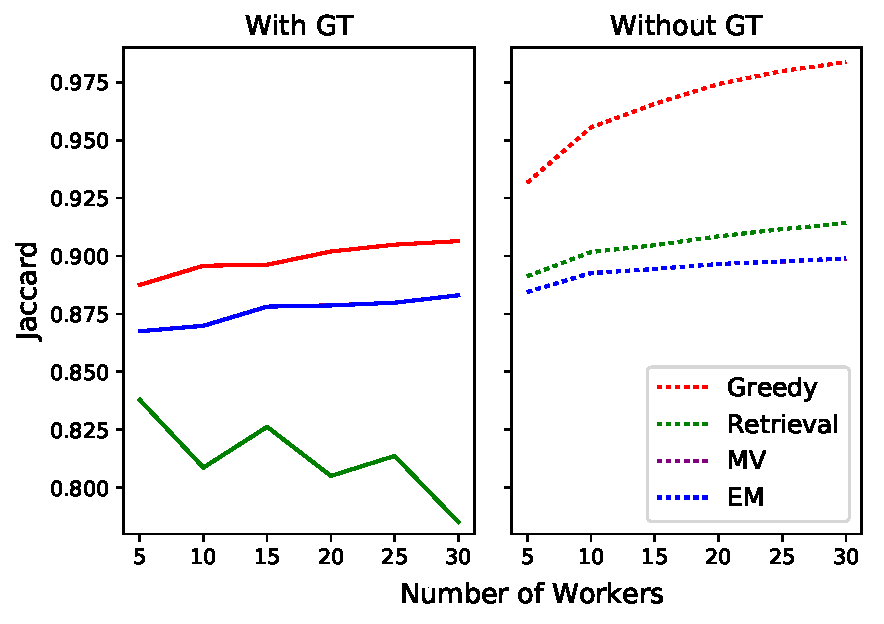
\includegraphics[trim={0 5pt 4pt 0},clip,width=0.8\textwidth]{plots/Retrieval_vs_Aggregation.pdf}
   \vspace{-4pt}
   \caption{Performance of the original algorithms that do not make use of ground truth information (Left) and ones that do (Right). MV and EM results are so close that they overlay on each other.} %\agp{Explain setup for this. How did you generate this?} \dor{not sure what aditya means?}}%Performance comparison between best-performing retrieval and aggregation-based methods. 
   \label{retrieval_vs_aggregation}   
   \vspace{-10pt}
   \setlength{\abovecaptionskip}{-30pt}
   \setlength{\belowcaptionskip}{-23pt}
\end{figure} 
\npar In Figure~\ref{retrieval_vs_aggregation}, we vary the number of worker segmentations along the x-axis and plot the average Jaccard score for a given algorithm across different worker samples of a given size in the y-axis. Figure~\ref{retrieval_vs_aggregation} (left) shows that the performance of aggregation-based algorithms (greedy, EM) exceeds the best-achievable through existing retrieval-based method (num pts). In Figure \ref{retrieval_vs_aggregation} (right), we estimate the upper-bound performance of each algorithm by assuming that `full information' based on ground truth was given to the algorithm. For greedy, the algorithm is aware of all the actual tile overlap and non-overlap areas against ground truth, and does not need to approximate these values. For EM, we look at the performance of the algorithm if the true worker quality parameter values (under our chosen worker quality model) are known. For retrieval, the full information version directly picks the worker with the highest Jaccard with respect to the ground truth segmentation. By making use of ground truth information (Figure~\ref{retrieval_vs_aggregation} right), the best aggregation-based algorithm can achieve a close-to-perfect average Jaccard score of 0.98 as an upper bound, far exceeding the results achievable by any single `best' worker (J=0.91). This result demonstrates that aggregation-based methods are able to achieve better performance by performing inference at the tile granularity, which is guaranteed to be finer than any individual worker segmentation. 

\stitle{The performance of aggregation-based methods scale well as more worker segmentations are added.}
\par \noindent Intuitively, larger numbers of worker segmentations result in finer granularity tiles for the aggregation-based methods. The first row in Table~\ref{statsTable} lists the average percentage change in Jaccard between 5-workers and 30-workers samples, demonstrating a monotonically increasing relationship between number of worker segmentations used and the performance. However, retrieval-based methods do not benefit from more segmentations.

\stitle{Experiment 2: Clustering as preprocessing improves algorithmic performance.}
\par \noindent The average percentage change between the no clustering and clustering results is shown in Table~\ref{statsTable}. Clustering generally results in an accuracy increase. Since the `full information' variants are already free of semantic ambiguity and errors, clustering does not results in further improvement. %In particular, we see a greater improvement with clustering preprocessing for algorithms that are not very robust in resolving semantic errors or ambiguity, such as for the \texttt{num pts} retrieval algorithm, than compared to the aggregation-based methods. 
%\agp{Weird, this is experiment 2. Divide this up into two parts. (Right now it seems as if all findings are from Fig 4, so this comes as a surprise.)}\dor{should we divide table~\ref{statsTable} into two separate tables?}
\begin{table}[h!]
   \small
     \setlength\tabcolsep{1.5pt}
      \begin{tabular}{l|l|l|l|l|l|l}
         & \multicolumn{2}{c|}{Retrieval-based} & \multicolumn{4}{l}{Aggregation-based} \\ \hline
      Algorithm         & num pts         & worker*        & MV    & EM    & greedy  & greedy*  \\ \hline
      Worker Scaling    & -6.30           & 2.58               & 1.63  & 1.64  & 2.16    & 5.59         \\ \hline
      Clustering Effect & 5.92            & -0.02              & 2.05  & 1.38  & 5.55    & -0.06       
      \end{tabular}
      \caption{Percentage change due to worker scaling and clustering. Algorithms with * makes use of ground truth information.}
      \label{statsTable}
\end{table}